\section{The Cross Product}\label{sec:cross_product}

``Orthogonality'' is immensely important. A quick scan of your current environment will undoubtedly reveal numerous surfaces and edges that are perpendicular to each other (including the edges of this page). The dot product provides a quick test for orthogonality:  vectors $\vec u$ and $\vec v$ are perpendicular if, and only if, $\dotp uv=0$. 

Given two non--parallel, nonzero vectors $\vec u$ and $\vec v$ in space, it is very useful to find a vector $\vec w$ that is perpendicular to both $\vec u$ and $\vec v$. There is a operation, called the \textbf{cross product}, that creates such a vector. This section defines the cross product, then explores its properties and applications.

\definition{def:cross_product}{Cross Product}
{Let $\vec u =\la u_1,u_2,u_3\ra$ and $\vec v = \la v_1,v_2,v_3\ra$ be vectors in $\mathbb{R}^3$. The \textbf{cross product of $\vec u$ and $\vec v$}, denoted $\crossp uv$, is the vector
\index{vectors!cross product}\index{cross product!definition}
$$\crossp uv = \la u_2v_3-u_3v_2,-(u_1v_3-u_3v_1),u_1v_2-u_2v_1\ra.$$
}

This definition can be a bit cumbersome to remember. After an example we will give a convenient method for computing the cross product. For now, careful examination of the products and differences given in the definition should reveal a pattern that is not too difficult to remember. (For instance, in the first component only 2 and 3 appear as subscripts; in the second component, only 1 and 3 appear as subscripts. Further study reveals the order in which they appear.)

Let's practice using this definition by computing a cross product.\\

\example{ex_crossp1}{Computing a cross product}{
Let $\vec u = \la 2,-1,4\ra$ and $\vec v = \la 3,2,5\ra$. Find $\crossp uv$, and verify that it is orthogonal to both $\vec u$ and $\vec v$.
}
{Using Definition \ref{def:cross_product}, we have
$$\crossp uv = \la (-1)5-(4)2,-\big((2)5-(4)3\big), (2)2-(-1)3\ra = \la -13,2,7\ra.$$ 
(We encourage the reader to compute this product on their own, then verify their result.)

\enlargethispage{2\baselineskip}
We test whether or not $\crossp uv$ is orthogonal to $\vec u$ and $\vec v$ using the dot product:
$$\big(\crossp uv\big) \cdot \vec u = \la -13,2,7\ra \cdot \la 2,-1,4\ra = 0,$$
$$\big(\crossp uv\big) \cdot \vec v = \la -13,2,7\ra \cdot \la 3,2,5 \ra = 0.$$
Since both dot products are zero, $\crossp uv$ is indeed orthogonal to both $\vec u$ and $\vec v$.
}\\

A convenient method of computing the cross product starts with forming a particular $3\times 3$ \emph{matrix}, or rectangular array. The first row comprises the standard unit vectors $\vec i$, $\vec j$, and $\vec k$. The second and third rows are the vectors $\vec u$ and $\vec v$, respectively. Using $\vec u$ and $\vec v$ from Example \ref{ex_crossp1}, we begin with:

\btz [baseline=-3pt,>=stealth]
\node at (0,0) {$\begin{array}{ccc} \veci&\vecj&\veck \\  2&-1&4\\3&2&5\end{array}$};
\etz

Now repeat the first two columns after the original three:
\btz [baseline=-3pt,>=stealth]
\node at (0,0) {$\begin{array}{ccccc} \veci&\vecj&\veck&\veci&\vecj \\  2&-1&4&2&-1\\3&2&5&3&2\end{array}$};
\etz

This gives three full ``upper left to lower right'' diagonals, and three full ``upper right to lower left'' diagonals, as shown. Compute the products along each diagonal, then add the products on the right and subtract the products on the left:

\btz [baseline=-3pt,>=stealth]
\node at (0,0) {$\begin{array}{ccccc} \ \veci\ &\ \vecj\ &\ \veck\ &\ \veci\ &\ \vecj\ \\  2&-1&4&2&-1\\3&2&5&3&2\end{array}$};
\draw[->,  thin] (-1.3,.4) -- (.5,-.8) node[below right] {$-5\veci$};
\draw[->,  thin] (-.7,.4) -- (1.3,-.8) node[below right ] {12\vecj};
\draw[->, thin] (0,.4) -- (2,-.8) node[below right] {4\veck};
\draw[->, thin] (0,.4) -- (-2,-.8) node[below left] {$-3\veck$};
\draw[->, thin] (.7,.4) -- (-1.3,-.8) node[below left ] {8\veci};
\draw[->, thin] (1.3,.4) -- (-.5,-.8) node[below left] {10\vecj};
\etz
$$\crossp uv = \big(-5\veci+12\vecj+4\veck\,\big) - \big(-3\veck+8\veci+10\vecj\,\big) = -13\veci+2\vecj+7\veck = \la -13,2,7\ra.$$

We practice using this method.\\

\example{ex_crossp2}{Computing a cross product}{
Let $\vecu=\la 1,3,6\ra$ and $\vec v = \la -1,2,1\ra$. Compute both $\crossp uv$ and $\crossp vu$.}
{To compute $\crossp uv$, we form the matrix as prescribed above, complete with repeated first columns:
$$\begin{array}{ccccc} \ \veci\ &\ \vecj\ &\ \veck\ &\ \veci\ &\ \vecj\ \\  1&3&6&1&3\\-1&2&1&-1&2\end{array}$$
We let the reader compute the products of the diagonals; we give the result:
$$\crossp uv = \big(3\veci-6\vecj+2\veck\,\big) - \big(-3\veck + 12\veci+\vecj\,\big) = \la -9,-7,5\ra.$$

To compute $\crossp vu$, we switch the second and third rows of the above matrix, then multiply along diagonals and subtract:

$$\begin{array}{ccccc} \ \veci\ &\ \vecj\ &\ \veck\ &\ \veci\ &\ \vecj\ \\-1&2&1&-1&2\\  1&3&6&1&3\end{array}$$
Note how with the rows being switched, the products that once appeared on the right now appear on the left, and vice--versa. Thus the result is:
$$\crossp vu = \big(12\veci+\vecj-3\veck\,\big) - \big(2\veck + 3\veci-6\vecj\,\big) = \la 9,7,-5\ra,$$
which is the opposite of $\crossp uv$. We leave it to the reader to verify that each of these vectors is orthogonal to $\vec u$ and $\vec v$.
}\\

\noindent\textbf{\large Properties of the Cross Product}\\

It is not coincidence that $\crossp vu = -(\crossp uv)$ in the preceding example; one can show using Definition \ref{def:cross_product} that this will always be the case. The following theorem states several useful properties of the cross product, each of which can be verified by referring to the definition.

\setboxwidth{15pt}
%\noindent\hskip-50pt\begin{minipage}{\linewidth}
\theorem{thm:cross_prod_prop}{Properties of the Cross Product}
{Let $\vecu$, $\vecv$ and $\vecw$ be vectors in $\mathbb{R}^3$ and let $c$ be a scalar. The following identities hold:
\index{vectors!cross product}\index{cross product!properties}
\begin{enumerate}
	\item \parbox{167pt}{$\crossp uv = -(\crossp vu)$} Anticommutative Property
	\item	\begin{enumerate}
		\item \parbox{145pt}{$(\vec u+\vec v)\times \vecw = \crossp uw+\crossp vw$} Distributive Properties
		\item	$\vec u \times (\vec v+\vec w) = \crossp uv+\crossp uw$
	\end{enumerate}
	\item		$c(\crossp uv) = (c\vecu) \times \vec v = \vecu \times (c\vecv)$
	\item		\begin{enumerate}
		\item \parbox{145pt}{$(\crossp uv)\cdot \vecu = 0$} Orthogonality Properties
		\item	$(\crossp uv)\cdot \vecv = 0$
	\end{enumerate}
	\item		$\crossp uu = \vec 0$
	\item		$\crossp u0 = \vec 0$
	\item		\parbox{167pt}{$\vecu \cdot (\vecv\times\vecw) = (\crossp uv)\cdot \vecw$} Triple Scalar Product
\end{enumerate}
}
%\end{minipage}
\restoreboxwidth

We introduced the cross product as a way to find a vector orthogonal to two given vectors, but we did not give a proof that the construction given in Definition \ref{def:cross_product} satisfies this property. Theorem \ref{thm:cross_prod_prop} asserts this property holds; we leave it as a problem in the Exercise section to verify this.

Property 5 from the theorem is also left to the reader to prove in the Exercise section, but it reveals something more interesting than ``the cross product of a vector with itself is $\vec 0$.'' Let $\vec u$ and $\vec v$ be parallel vectors; that is, let there be a scalar $c$ such that $\vecv = c\vecu$. Consider their cross product:
\begin{align*}
\crossp uv &= \vecu \times (c\vec u) \\
					&=	\parbox{50pt}{$c(\crossp uu)$}\text{(by Property 3 of Theorem \ref{thm:cross_prod_prop})}\\
					&= \parbox{50pt}{$\vec 0$.}\text{(by Property 5 of Theorem \ref{thm:cross_prod_prop})}
\end{align*}

We have just shown that the cross product of parallel vectors is $\vec 0$. This hints at something deeper. Theorem \ref{thm:dot_product} related the angle between two vectors and their dot product; there is a similar relationship relating the cross product of two vectors and the angle between them, given by the following theorem.

\theorem{thm:cross_product}{The Cross Product and Angles}
{Let $\vec u$ and $\vec v$ be nonzero vectors in $\mathbb{R}^3$. Then
$$\norm{\crossp uv} = \vnorm u\, \vnorm v \sin\theta,$$
where $\theta$, $0\leq \theta \leq \pi$, is the angle between $\vecu$ and $\vecv$.
\index{vectors!cross product}\index{cross product!properties}
}

\mnote{.52}{\textbf{Note:} We could rewrite Definition \ref{def:orthogonal} and Theorem \ref{thm:cross_product} to include $\vec 0$, then define that $\vec u$ and $\vec v$ are parallel if $\vec u\times\vec v=\vec 0$. Since $\vec 0\cdot \vec v =0$ and $\vec 0\times \vec v = \vec 0$, this would mean that $\vec 0$ is both parallel \emph{and} orthogonal to all vectors.
%Definition \ref{def:orthogonal} (through Theorem \ref{thm:dot_product}) defines $\vec u$ and $\vec v$ to be orthogonal if $\vec u\cdot\vec v=\vec 0$. We could rewrite Theorem \ref{thm:cross_product} to include $\vec 0$, then define that $\vec u$ and $\vec v$ are parallel if $\vec u\times \vec v =\vec 0$. By such a definition, $\vec 0$ would be both orthogonal and parallel to every vector. 
Apparent paradoxes such as this are not uncommon in mathematics and can be very useful. (See also the marginal note on page \pageref{note:parallel}.)\label{note:crossp}}
Note that this theorem makes a statement about the \emph{magnitude} of the cross product. When the angle between $\vecu$ and $\vecv$ is 0 or $\pi$ (i.e., the vectors are parallel), the magnitude of the cross product is 0. The only vector with a magnitude of 0 is $\vec 0$ (see Property \ref{thm:zero_norm} of Theorem \ref{thm:vector_properties}), hence the cross product of  parallel vectors is $\vec 0$.\\

We demonstrate the truth of this theorem in the following example.\\

\example{ex_crossp3}{The cross product and angles}{
Let $\vec u = \la 1,3,6\ra$ and $\vec v = \la -1,2,1\ra$ as in Example \ref{ex_crossp2}. Verify Theorem \ref{thm:cross_product} by finding $\theta$, the angle between $\vecu$ and $\vecv$, and the magnitude of $\crossp uv$.}
{We use Theorem \ref{thm:dot_product} to find the angle between $\vecu$ and $\vecv$. 
\begin{align*}
\theta &= \cos^{-1}\left(\frac{\dotp uv}{\vnorm u\, \vnorm v}\right) \\
			&= \cos^{-1}\left(\frac{11}{\sqrt{46}\sqrt{6}}\right)\\
			&\approx 0.8471 = 48.54^\circ.
\end{align*}

Our work in Example \ref{ex_crossp2} showed that $\crossp uv = \la -9,-7,5\ra$, hence $\norm{\crossp uv} = \sqrt{155}.$ Is $\norm{\crossp uv} = \vnorm u\, \vnorm v\sin\theta$? Using numerical approximations, we find:
\begin{align*}
\norm{\crossp uv} &=\sqrt{155}  & \vnorm u\,\vnorm v \sin\theta & = \sqrt{46}\sqrt{6}\sin 0.8471\\
									&\approx 12.45. & &\approx 12.45.
\end{align*}
Numerically, they seem equal. Using a right triangle, one can show that 
$$\sin\left(\cos^{-1}\left(\frac{11}{\sqrt{46}\sqrt{6}}\right)\right) = \frac{\sqrt{155}}{\sqrt{46}\sqrt{6}},$$ which allows us to verify the theorem exactly.
}\\

\noindent\textbf{Right Hand Rule}\\

The anticommutative property of the cross product demonstrates that $\crossp uv$ and $\crossp vu$ differ only by a sign -- these vectors have the same magnitude but point in the opposite direction. When seeking a vector perpendicular to $\vec u$ and $\vec v$, we essentially have two directions to choose from, one in the direction of $\crossp uv$ and one in the direction of $\crossp vu$. Does it matter which we choose? How can we tell which one we will get without graphing, etc.?

Another wonderful property of the cross product, as defined, is that it follows the \textbf{right hand rule.} Given $\vec u$ and $\vec v$ in $\mathbb{R}^3$ with the same initial point, point the index finger of your right hand in the direction of $\vecu$ and let your middle finger point in the direction of $\vecv$ (much as we did when establishing the right hand rule for the 3-dimensional coordinate system). Your thumb will naturally extend in the direction of $\crossp uv$. One can ``practice'' this using Figure \ref{fig:crossp_rhr}. If you switch, and point the index finder in the direction of $\vecv$ and the middle finger in the direction of $\vecu$, your thumb will now point in the opposite direction, allowing you to ``visualize'' the anticommutative property of the cross product.
\mfigurethree{width=150pt,3Dmenu,activate=onclick,deactivate=onclick,
3Droll=0,
3Dortho=0.0044,
3Dc2c=.78 .32 .53,
3Dcoo=0 0 34,
3Droo=150,
3Dlights=Headlamp,add3Djscript=asylabels.js}{}{.5}{Illustrating the Right Hand Rule of the cross product.}{fig:crossp_rhr}{figures/figcrossp_rhr}
%\mfigure[scale=1.25,trim=5mm 5mm 5mm 5mm,clip=true]{.5}{Illustrating the Right Hand Rule of the cross product.}{fig:crossp_rhr}{figures/figcrossp_rhr}

\vskip\baselineskip
\noindent\textbf{\large Applications of the Cross Product}\\

There are a number of ways in which the cross product is useful in mathematics, physics and other areas of science beyond ``just'' finding a vector perpendicular to two others. We highlight a few here.\index{cross product!applications}\\
%\enlargethispage{\baselineskip}
%\clearpage\enlargethispage{2\baselineskip}

\noindent\textbf{Area of a Parallelogram}\\

It is a standard geometry fact that the area of a parallelogram is $A = bh$, where $b$ is the length of the base and $h$ is the height of the parallelogram, as illustrated in Figure \ref{fig:crossp_parallelogram}(a). As shown when defining the Parallelogram Law of vector addition, two vectors $\vecu$ and $\vecv$ define a parallelogram when drawn from the same initial point, as illustrated in Figure \ref{fig:crossp_parallelogram}(b). Trigonometry tells us that $h = \vnorm u \sin \theta$, hence the area of the parallelogram is 
\begin{equation}A = \vnorm u\,\vnorm v\sin\theta = \norm{\crossp uv},\label{eq:crossp1}\end{equation}
where the second equality comes from Theorem \ref{thm:cross_product}.
\mtable{.75}{Using the cross product to find the area of a parallelogram.}{fig:crossp_parallelogram}{%
\begin{tabular}{c}
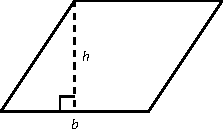
\includegraphics{figures/figcrossp_parallelogram1}\\
(a) \\[15pt]
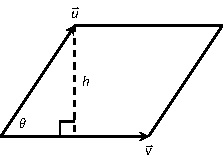
\includegraphics{figures/figcrossp_parallelogram2}\\
(b) \\
\end{tabular}
}
We illustrate using Equation \eqref{eq:crossp1} in the following example.
\index{cross product!applications!area of parallelogram}\\

\example{ex_crossp4}{Finding the area of a parallelogram}{
\begin{enumerate}
	\item Find the area of the parallelogram defined by the vectors $\vecu = \la 2,1\ra$ and $\vecv = \la 1,3\ra$.
	\item	Verify that the points $A = (1,1,1)$, $B = (2,3,2)$, $C = (4,5,3)$ and $D = (3,3,2)$ are the vertices of a parallelogram. Find the area of the parallelogram.
\end{enumerate}
}
{\begin{enumerate}
	\item Figure \ref{fig:crossp4}(a) sketches the parallelogram defined by the vectors $\vec u$ and $\vec v$. We have a slight problem in that our vectors exist in $\mathbb{R}^2$, not $\mathbb{R}^3$, and the cross product is only defined on vectors in $\mathbb{R}^3$. We skirt this issue by viewing $\vec u$ and $\vecv$ as vectors in the $x-y$ plane of $\mathbb{R}^3$, and rewrite them as $\vec u = \la 2,1,0\ra$ and $\vecv =\la 1,3,0\ra$. We can now compute the cross product. 
	It is easy to show that $\crossp uv = \la 0,0,5\ra$; therefore the area of the parallelogram is $A = \norm{\crossp uv} = 5$.
	\mtable{.35}{Sketching the parallelograms in Example \ref{ex_crossp4}.}{fig:crossp4}{%
	\begin{tabular}{c}
	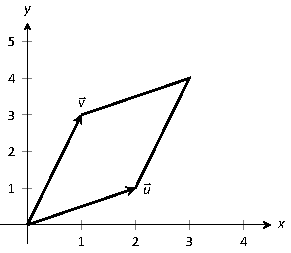
\includegraphics{figures/figcrossp4b}\\
	(a)\\[15pt]
	\myincludegraphicsthree{width=125pt,3Dmenu,activate=onclick,deactivate=onclick,
3Droll=0,
3Dortho=0.004,
3Dc2c=.42 .87 .26,
3Dcoo=61 60 63,
3Droo=250,
3Dlights=Headlamp,add3Djscript=asylabels.js}{scale=1.25,trim=4mm 5mm 4mm 5mm,clip=true}{figures/figcrossp4a}\\
	%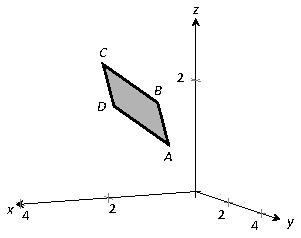
\includegraphics{figures/figcrossp4a}\\
	(b)
	\end{tabular}
	}
	\item		To show that the quadrilateral $ABCD$ is a parallelogram (shown in Figure \ref{fig:crossp4}(b)), we need to show that the opposite sides are parallel. We can quickly show that $\vv{AB} =\vv{DC} = \la 1,2,1\ra$ and $\vv{BC} = \vv{AD} = \la 2,2,1\ra$. We find the area by computing the magnitude of the cross product of $\vv{AB}$ and $\vv{BC}$:
	$$\vv{AB} \times \vv{BC} = \la 0,1,-2\ra \quad \Rightarrow \quad \norm{\vv{AB}\times\vv{BC}} = \sqrt{5} \approx 2.236.$$
\end{enumerate}
\vskip-\baselineskip
}\\

This application is perhaps more useful in finding the area of a triangle (in short, triangles are used more often than parallelograms). We illustrate this in the following example.\\

\example{ex_crossp5}{Area of a triangle}{
Find the area of the triangle with vertices $A=(1,2)$, $B=(2,3)$ and $C=(3,1)$, as pictured in Figure \ref{fig:crossp5}.}
{We found the area of this triangle in Example \ref{ex_abc4} to be $1.5$ using integration. There we discussed the fact that finding the area of a triangle can be inconvenient using the ``$\frac12bh$'' formula as one has to compute the height, which generally involves finding angles, etc. Using a cross product is much more direct.
\mfigure{.78}{Finding the area of a triangle in Example \ref{ex_crossp5}.}{fig:crossp5}{figures/figcrossp5}

We can choose any two sides of the triangle to use to form vectors; we choose $\vv{AB} = \la 1,1\ra$ and $\vv{AC}=\la 2,-1\ra$. As in the previous example, we will rewrite these vectors with a third component of 0 so that we can apply the cross product. The area of the triangle is
$$\frac12\norm{\vv{AB}\times\vv{AC}} = \frac12\norm{\la 1,1,0\ra \times \la 2,-1,0\ra} = \frac12\norm{\la 0,0,-3\ra} = \frac32.$$
We arrive at the same answer as before with less work.
}\\

\noindent\textbf{Volume of a Parallelepiped}

The three dimensional analogue to the parallelogram is the \textbf{parallelepiped}. Each face is parallel to the opposite face, as illustrated in Figure \ref{fig:crossp_parallelepiped}. By crossing $\vec v$ and $\vec w$, one gets a vector whose magnitude is the area of the base. Dotting this vector with $\vecu$ computes the volume of parallelepiped! (Up to a sign; take the absolute value.)
\mnote{.5}{\textbf{Note:} The word ``parallelepiped'' is pronounced ``parallel--eh--pipe--ed.''}
\mfigurethree{width=100pt,3Dmenu,activate=onclick,deactivate=onclick,
3Droll=0,
3Dortho=0.0045,
3Dc2c=.84 .46 .26,
3Dcoo=0 110 86,
3Droo=150,
3Dlights=Headlamp,add3Djscript=asylabels.js}{}{.35}{A parallelepiped is the three dimensional analogue to the parallelogram.}{fig:crossp_parallelepiped}{figures/figcrosspparallelpiped}
%\mfigure{.53}{A parallelepiped is the three dimensional analogue to the parallelogram.}{fig:crossp_parallelepiped}{figures/figcrosspparallelpiped}
\index{cross product!applications!volume of parallelepiped}

Thus the volume of a parallelepiped defined by vectors $\vecu$, $\vecv$ and $\vec w$ is \begin{equation}V = |\vecu\cdot (\crossp vw)|.\label{eq:crossp2}\end{equation}
Note how this is the Triple Scalar Product, first seen in Theorem \ref{thm:cross_prod_prop}. Applying the identities given in the theorem shows that we can apply the Triple Scalar Product in any ``order'' we choose to find the volume. That is,
$$V = |\vecu\cdot(\crossp vw)| = |\vec u\cdot (\crossp wv)| = |(\crossp uv)\cdot \vecw|,\quad \text{etc.}$$

\example{ex_crossp6}{Finding the volume of parallelepiped}{
Find the volume of the parallepiped defined by the vectors $\vecu = \la 1,1,0\ra$, $\vecv = \la -1,1,0\ra$ and $\vecw = \la 0,1,1\ra$. 
}
{We apply Equation \eqref{eq:crossp2}. We first find $\crossp vw =\la 1,1,-1\ra$. Then
$$|\vec u\cdot(\crossp vw)| = |\la 1,1,0\ra \cdot \la1,1,-1\ra| = 2.$$
So the volume of the parallelepiped is 2 cubic units.
\mfigurethree{width=125pt,3Dmenu,activate=onclick,deactivate=onclick,
3Droll=0,
3Dortho=0.0045,
3Dc2c=4 4 2,
3Dcoo=0 50 50,
3Droo=150,
3Dlights=Headlamp,add3Djscript=asylabels.js}{}{.8}{A parallelepiped in Example \ref{ex_crossp6}.}{fig:crossp6}{figures/figcrossp6}
%\mfigure{.3}{A parallelepiped in Example \ref{ex_crossp6}.}{fig:crossp6}{figures/figcrossp6}
}\\

While this application of the Triple Scalar Product is interesting, it is not used all that often: parallelepipeds are not a common shape in physics and engineering. The last application of the cross product is very applicable in engineering.\\

\noindent\textbf{Torque}\\

\textbf{Torque} is a measure of the turning force applied to an object. A classic scenario involving torque is the application of a wrench to a bolt. When a force is applied to the wrench, the bolt turns. When we represent the force and wrench with vectors $\vec F$ and $\vec \ell$, we see that the bolt moves (because of the threads) in a  direction orthogonal to $\vec F$ and $\vec \ell$. Torque is usually represented by the Greek letter $\tau$, or tau, and has units of N$\cdot$m, a Newton--meter, or ft$\cdot$lb, a foot--pound.\index{cross product!applications!torque}

While a full understanding of torque is beyond the purposes of this book, when a force $\vec F$ is applied to a lever arm $\vec \ell$, the resulting torque is \begin{equation}\vec \tau = \crossp \ell F.\label{eq:crossp3}\end{equation}

\example{ex_crossp7}{Computing torque}{
A lever of length 2ft makes an angle with the horizontal of $45^\circ$. Find the resulting torque when a force of 10lb is applied to the end of the level where:
\mfigure{.5}{Showing a force being applied to a lever in Example \ref{ex_crossp7}.}{fig:crossp7}{figures/figcrossp7}
\begin{enumerate}
	\item the force is perpendicular to the lever, and
	\item	the force makes an angle of $60^\circ$ with the lever, as shown in Figure \ref{fig:crossp7}.
\end{enumerate}
}
{\begin{enumerate}
	\item We start by determining vectors for the force and lever arm. Since the lever arm makes a $45^\circ$ angle with the horizontal and is 2ft long, we can state that $\vec \ell = 2\la \cos 45^\circ,\sin 45^\circ\ra = \la \sqrt2,\sqrt2\ra.$
	
	Since the force vector is perpendicular to the lever arm (as seen in the left hand side of Figure \ref{fig:crossp7}), we can conclude it is making an angle of $-45^\circ$ with the horizontal. As it has a magnitude of 10lb, we can state $\vec F = 10\la \cos (-45^\circ), \sin(-45^\circ)\ra = \la 5\sqrt2,-5\sqrt2\ra.$
	
	Using Equation \eqref{eq:crossp3} to find the torque requires a cross product. We again let the third component of each vector be 0  and compute the cross product:
	\begin{align*}
	\vec\tau &= \crossp \ell F \\
				&= \la \sqrt2,\sqrt2,0\ra \times \la 5\sqrt2,-5\sqrt2,0\ra \\
				&= \la 0,0,-20\ra
	\end{align*}
	This clearly has a magnitude of 20 ft-lb.
	
	We can view the force and lever arm vectors as lying ``on the page''; our computation of $\vec\tau$ shows that the torque goes ``into the page.'' This follows the Right Hand Rule of the cross product, and it also matches well with the example of the wrench turning the bolt. Turning a bolt clockwise moves it in.
	
	\item		Our lever arm can still be represented by $\vec \ell = \la \sqrt2,\sqrt2\ra$. As our force vector makes a $60^\circ$ angle with $\vec \ell$, we can see (referencing the right hand side of the figure) that $\vec F$ makes a $-15^\circ$ angle with the horizontal. Thus 
	\begin{align*}
	\vec F = 10\la \cos-15^\circ,\sin-15^\circ\ra &= \la \frac{5(1+\sqrt3)}{\sqrt2},\frac{5(-1+\sqrt3)}{\sqrt2}\ra \\
	&\approx \la 9.659,-2.588\ra.\end{align*}
	
	We again make the third component 0 and take the cross product to find the torque:
	\begin{align*}
	\vec\tau &= \crossp \ell F\\
					&= \la \sqrt2,\sqrt2,0\ra \times  \la \frac{5(1+\sqrt3)}{\sqrt2},\frac{5(-1+\sqrt3)}{\sqrt2},0\ra\\
					&= \la 0,0,-10\sqrt3\ra\\
					&\approx \la 0,0,-17.321\ra.
	\end{align*}
	As one might expect, when the force and lever arm vectors \textit{are} orthogonal, the magnitude of force is greater than when the vectors \textit{are not} orthogonal.
\end{enumerate}
\vskip-\baselineskip
}\\

While the cross product has a variety of applications (as noted in this chapter), its fundamental use is finding a vector perpendicular to two others. Knowing a vector is orthogonal to two others is of incredible importance, as it allows us to find the equations of lines and planes in a variety of contexts. The importance of the cross product, in some sense, relies on the importance of lines and planes, which see widespread use throughout engineering, physics and mathematics. We study lines and planes in the next two sections. 

\printexercises{exercises/10_04_exercises}

